\documentclass{article}
\usepackage[a4paper, left=2cm, right=2cm, top=3cm, bottom=3cm, headheight=35pt, includehead]{geometry}

\usepackage[english]{babel}
\usepackage[utf8]{inputenc}
\usepackage{fancyhdr}

\usepackage{enumitem}
\usepackage{amsmath}
\usepackage{mathtools}
\usepackage{listings}


\usepackage{tikz}
\usetikzlibrary{arrows.meta}


\lstset{mathescape=true,
		morekeywords={if,else,and,then,for,return}}

\pagestyle{fancy}
\fancyhf{}
\lhead{\today \\ Andrés Montoya, 405409 \\ Laura Koch, 406310 }
\chead{Introduction to Artificial Intelligence \\ Assignment 02}
\rhead{ Lennart Holzenkamp, 407761 \\ Simon Michau, 406133 \\ Til Mohr, 405959}

\begin{document}

\section*{Exercise 2.1}
\begin{enumerate}[label=(\alph*)]
	\item	$g(n)$ denotes the path cost from the root of the search tree to node $n$. Since the Greedy Search always expands the node $n^*$ where $h(n^*) = g(n^*)$ is minimal, the resulting algorithm can be described as a shortest path search (or lowest cost search) algorithm.
	\item	Since $d(n)$ denotes the depth of a node $n$ in the search tree and the Greedy Search always expands the node $n^*$ where $h(n^*) = d(n^*)$ is minimal (so minimal depth), the resulting algorithm is a BFS.
	\item	$\frac{1}{1+d(n)}$ is inversely proportional to the depth of node $n$ in the search tree. Therefore, the Greedy Search always expands the node $n^*$ with the largest depth. So we get an DFS algorithm.
\end{enumerate}

\section*{Exercise 2.2}
\subsection*{1)}
An admissible heuristic is a function that never overestimates the cost of the minimum cost path from a node to the goal node. Let $h^*(n)$ be the optimal cost to reach the goal from $n$. If $h$ is admissible, then $\forall n: h(n) \leq h^*(n)$.\\[2\baselineskip]
Let $h$ be consistent.\\
Suppose there is not path from $n$ to the goal state. Then $h^*(n) = \infty$, therefore $h(n) \leq h^*(n)$.\\
Now suppose that there is some path from $n$ to te goal state $g$. Let $(n, x_1, \dots, x_m, g)$ be the shortest path from $n$ to the goal state $g$ with corresponding actions $(a_n, a_{x_1}, \dots, a_{x_m})$.\\[2\baselineskip]
Induction:\\
Consider $x_m$. $h(x_m) \leq c(x_m, a_{x_m}, g) + h(g) \stackrel{h(g)=0}{=} c(x_m, a_{x_m}, g) = h^*(x_m)$.\\
Similarly $x_{m-1}$. $h(x_{m-1}) \leq c(x_{m-1}, a_{x_{m-1}}, x_m) + h(x_m) = c(x_{m-1}, a_{x_{m-1}}, x_m) + c(x_m, a_{x_m}, g) = h^*(x_{m-1})$.\\
By induction on the shortest past we get $h(n) \leq c(n, a_n, x_1)+ c(x_m, a_{x_m}, g) = h^*(n)$, which is of course the shortest path cost.\\[2\baselineskip]
Therefore when a heuristic is consistent, it is admissible.

\subsection*{2)}
Let there be the graph with goal node $G$:

\begin{figure}[htb]
\begin{minipage}[c]{.49\textwidth}
	\centering
	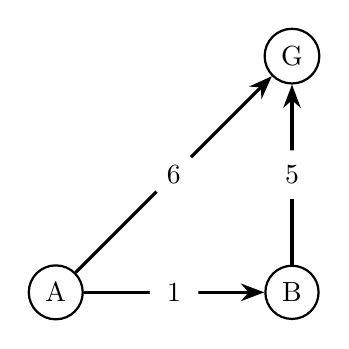
\begin{tikzpicture}
		\begin{scope}[every node/.style={circle,thick,draw}]
			\node (A) at (0,0) {A};
			\node (B) at (3,0) {B};
			\node (G) at (3,3) {G};
		\end{scope}

		\begin{scope}[>={Stealth[black]},
					every node/.style={fill=white,circle},
					every edge/.style={draw=black,very thick}]
			\path [->] (A) edge node {$1$} (B);
			\path [->] (B) edge node {$5$} (G);
			\path [->] (A) edge node {$6$} (G);
		\end{scope}
	\end{tikzpicture}
\end{minipage}
\begin{minipage}[c]{.49\textwidth}
	\centering
	\begin{tabular}{c|c}
		Node $n$ & $h^*(n)$ \\
		\hline
		A & 6 \\
		B & 5 \\
		G & 0
	\end{tabular}
\end{minipage}
\end{figure}

An admissible heuristic, that is not consistent:

\begin{center}
	\begin{tabular}{c|c}
		Node $n$ & $h(n)$ \\
		\hline
		A & 6 \\
		B & 1 \\
		G & 0
	\end{tabular}
\end{center}

\section*{Exercise 2.3}


\section*{Exercise 2.4}


\end{document}